\documentclass{report}

\input{scr/preamble}
\input{scr/macros}
\input{scr/letterfonts}

\title{\Huge{Solid State Physics}\\Tight-Binding Model Project}
\author{\huge{Zengxuan Liu}\\3042027511}
\date{\today}

\begin{document}

\maketitle
\newpage
% \pdfbookmark[<level>]{<title>}{<dest>}
\pdfbookmark[section]{\contentsname}{toc}
\tableofcontents
\pagebreak

\chapter{Simple 1D Tight-Binding Model}
\section{Task 1: Hamiltonian construction}

\qs{}{Write a program that constructs the Hamiltonian matrix in the periodic boundary conditions (PBC), where site $N$ is identified with site $0$.}

\qs{}{Modify the code to handle open boundary conditions (OBC), where sites $0$ and $N - 1$ are not connected.}

\dfn{Hamiltonian}{The Hamiltonian for the 1D tight-binding model is given by: $$H = -t \sum_n \Big(\ket{n + 1}\bra{n} + \ket{n}\bra{n + 1}\Big)$$}

\sol We are going to define the Hamiltonian matrix for the 1D tight-binding model under both periodic and open boundary conditions using the code block below:

\begin{lstlisting}
# PBC 
def pbc_Hamiltonian(n, t = 1):
    H = np.zeros((n, n))
    for i in range(n):
        H[i, (i + 1) % n] = -t
        H[(i + 1) % n, i] = -t
    return H

# OBC
def obc_Hamiltonian(n, t = 1):
    H = np.zeros((n, n))
    for i in range(n - 1):
        H[i, i + 1] = -t
        H[i + 1, i] = -t
    return H
\end{lstlisting}

\nt{$n$ is the number of lattice sites and $t$ is the hopping parameter. The key to ensure periodic boundary conditions is to use modulo arithmetic to connect the first and last lattice sites.}

\begin{Example}{Simple 1D Tight-Binding Model Hamiltonian in PBC and OBC}{}
    \begin{minipage}[t]{0.48\textwidth}
    \begin{lstlisting}[basicstyle=\ttfamily\scriptsize]
# Example
N = 5
H_PBC = pbc_Hamiltonian(N)
H_OBC = obc_Hamiltonian(N)

print("Hamiltonian in PBC:")
print(H_PBC)
print(scipy.linalg.ishermitian(H_PBC))
print("Hamiltonian in OBC:")
print(H_OBC)
print(scipy.linalg.ishermitian(H_OBC))



    \end{lstlisting}
    \end{minipage}
    \hfill
    \begin{minipage}[t]{0.48\textwidth}
    \begin{lstlisting}[basicstyle=\ttfamily\scriptsize]
Hamiltonian in PBC:
[[ 0. -1.  0.  0. -1.]
[-1.  0. -1.  0.  0.]
[ 0. -1.  0. -1.  0.]
[ 0.  0. -1.  0. -1.]
[-1.  0.  0. -1.  0.]]
True
Hamiltonian in OBC:
[[ 0. -1.  0.  0.  0.]
[-1.  0. -1.  0.  0.]
[ 0. -1.  0. -1.  0.]
[ 0.  0. -1.  0. -1.]
[ 0.  0.  0. -1.  0.]]
True
    \end{lstlisting}
    \end{minipage}
\end{Example}

\section{Task 2: Eigenvalue problem}
\setcounter{tcb@cnt@question}{0}

\qs{}{Diagonalize your Hamiltonian for both boundary conditions for $N = 100$. It is convenient to use \texttt{numpy.linalg.eigh()}.}

\sol Using \texttt{np.linalg.eigh()} to diagonalize the Hamiltonian:

\begin{lstlisting}
# Diagonalize
N = 100
E_PBC, psi_PBC = np.linalg.eigh(pbc_Hamiltonian(N))
E_OBC, psi_OBC = np.linalg.eigh(obc_Hamiltonian(N))
\end{lstlisting}

\nt{The outputs of \texttt{np.linalg.eigh()} are arrays of eigenvalues and respective eigenvectors, and the arrays are sorted in ascending order of eigenvalues.}

\qs{}{Plot the energy spectrum of both the periodic and open systems on the same figure. How similar or different are they? Is there a degeneracy in the periodic spectrum? What is the origin of this degeneracy? Does the open system break or preserve this degeneracy? Why?}


\sol Plotting the energy spectrum:

\begin{figure}[H]
    \centering
    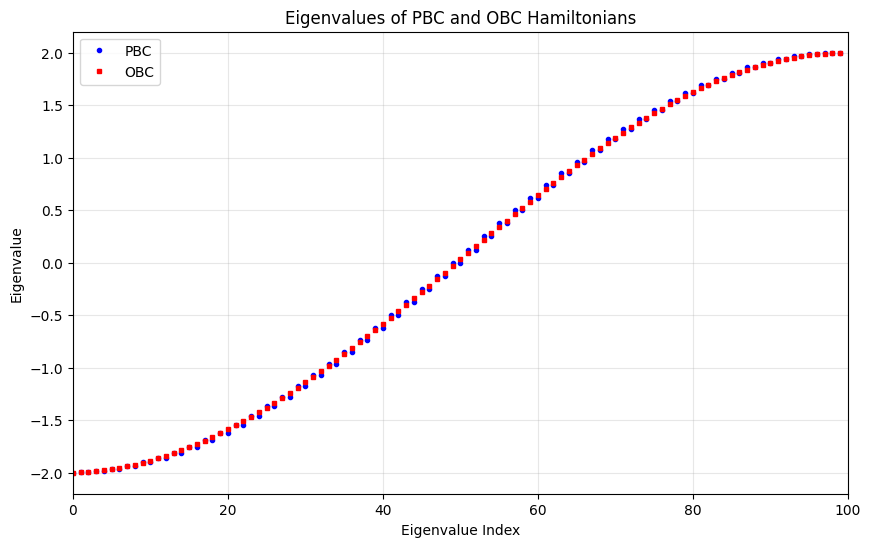
\includegraphics[width=0.45\textwidth]{fig/Question 1/Eigenvalues_PBC_OBC.png}
    \caption{Eigenvalues of PBC and OBC Hamiltonians}
\end{figure}

\begin{note}{}
    Consider the Hamiltonian and eigenvalue equation for a 1D tight-binding model:

    $$
        H = -t \sum_{n=1}^{N} \Big (\ket{n + 1} \bra{n} + \ket{n} \bra{n + 1} \Big ),\, H \ket{\psi} = E \ket{\psi}
    $$

    where $\ket{\psi} = \sum_{n=1}^{N} \psi_n \ket{n}$. Furthermore, we can express the eigenequation as:

    $$
        E \psi_n = -t (\psi_{n + 1} + \psi_{n - 1})
    $$

    \textbf{(a) PBC:} As common choice for periodic system, we can use plane wave eigenstates, we can write:

    $$ 
        \psi_n = \frac{1}{\sqrt{N}} e^{i k n}
    $$

    where $k = \frac{2\pi m}{N}$ for $m = 0, 1, \ldots, N-1$. Thus, we can substitute this into the eigenequation and find the corresponding eigenvalues:

    $$
        E(k) = -2t \cos(k) = -2t \cos\left(\frac{2\pi m}{N}\right)
    $$

    which shows the degeneracy that $E(k) = E(-k)$. 

    \textbf{(b) OBC:} For the open boundary conditions, we can use standing wave eigenstates, we can write:

    $$
        \psi_n = \sqrt{\frac{2}{N + 1}} \sin\left(\frac{m\pi n}{N + 1}\right)
    $$

    where $m = 1, 2, \ldots, N$. Thus, we can substitute this into the eigenequation and find the corresponding eigenvalues:

    $$
        E(m) = -2t \cos\left(\frac{m\pi}{N + 1}\right)
    $$

    \begin{itemize}
        \item Both systems have very similar spectra for $N = 100$.
        \item There is a degeneracy in the periodic system because of periodic boundary conditions. This periodicity maintains the translational symmetry which ensures that each atom has the same neighborhood environment. Therefore, this symmetry leads to degenerate energy levels.
        \item The open system breaks this degeneracy because the boundary conditions are different, leading to a unique energy spectrum for each state.
    \end{itemize}
\end{note}

\begin{question}{}{}
    \begin{enumerate}
        \item Plot the wave func1on probability distribu1on, $|\psi(x)|^2$, for the ground state and first two excited states of the \textbf{periodic} system as a func1on of posi1on and show them on the same plot. What do you notice about the first two excited states?
        \item Plot the wave func1on probability distribu1on, $|\psi_m(x)|^2$, for the ground state and first two excited states of the \textbf{open} system as a func1on of posi1on and show them on the same plot. What do you notice about the number of nodes?
    \end{enumerate}
\end{question}

\sol For 1D chains, the position can be represented by a discrete set of sites. Here, the position is indexed by $n$. Plotting the wave function probability distribution:

\begin{figure}[H]
    \centering

    \begin{minipage}{0.48\textwidth}
        \centering
        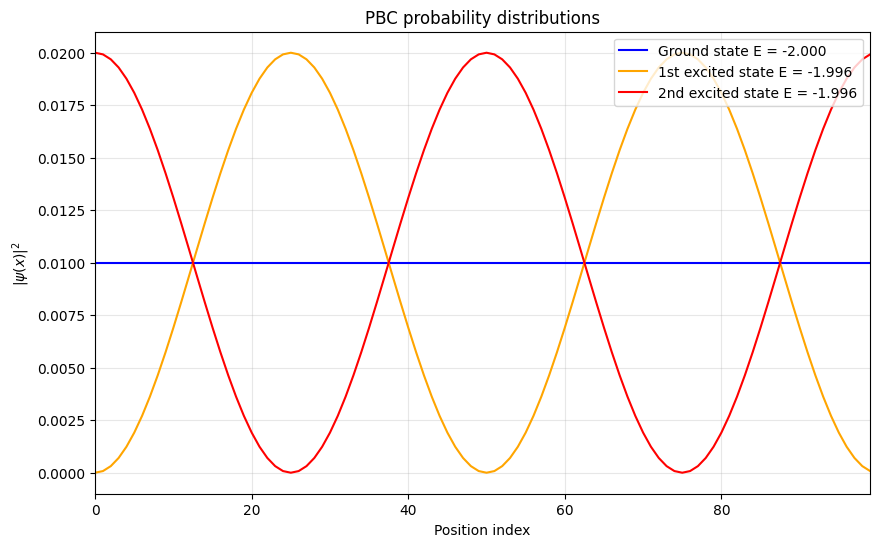
\includegraphics[width=\textwidth]{fig/Question 1/PBC_Prob_Distribution.png}
        \caption{Probability distribution for PBC system}
    \end{minipage}
    \hfill
    \begin{minipage}{0.48\textwidth}
        \centering
        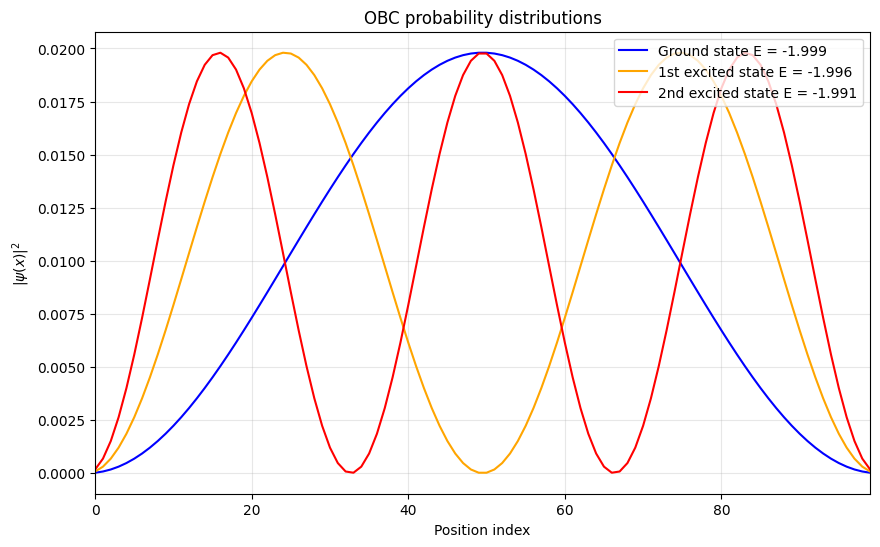
\includegraphics[width=\textwidth]{fig/Question 1/OBC_Prob_Distribution.png}
        \caption{Probability distribution for OBC system}
    \end{minipage}

\end{figure}

\begin{note}{}
    \begin{enumerate}
        \item PBC: The probability distribution for the ground state and first two excited states shows a periodic pattern due to the boundary conditions. For the first two excited states, they are degenerate and the wavefunctions are complex conjugates of each other, which leads to the same probability distribution shape for both states.
        \item OBC: The number of nodes in the probability distribution for the ground state and first two excited states are 0, 1, and 2 respectively, increasing with the energy level.
    \end{enumerate}
\end{note}

\chapter{The Su–Schrieffer–Heeger (SSH) model}
\section{Task 1: Hamiltonian construction}
\setcounter{tcb@cnt@question}{0}

\qs{}{Write a program to construct the Hamiltonian matrix for this system in both periodic and open boundary conditions. Make sure that there is an equal number of $A$ and $B$ sites.}

\dfnc{The Su–Schrieffer–Heeger (SSH) model}{The Su-Schrieffer-Heeger model describes a dimerized chain of $N$ unit cells with alterna1ng hopping magnitudes. The unit cell contains two sites ($A$ and $B$ sites), with intracell hopping $\nu$ and intercell hopping $\omega$. The Hamiltonian is given by $$ H = -\sum_{n = 0} \Big(\nu \ket{n; B}\bra{n; A} + \nu \ket{n; A}\bra{n; B}) + \omega \ket{n + 1; A}\bra{n; B}) + \omega \ket{n; B}\bra{n + 1; A}\Big) $$ where $n$ runs over all unit cells. In what follows, use $\omega = 1$ in your simulation.}

\sol We are going to define the Hamiltonian matrix for the SSH model in both periodic and open boundary conditions using the code block below:

\begin{lstlisting}
# PBC 
def pbc_Hamiltonian(n, nu, omega = 1):
    H = np.zeros((2 * n, 2 * n))
    for i in range(n):
        H[2 * i + 1, 2 * i] = -nu
        H[2 * i, 2 * i + 1] = -nu
        H[2 * (i + 1) % (2 * n), 2 * i + 1] = -omega
        H[2 * i + 1, 2 * (i + 1) % (2 * n)] = -omega
    return H

# OBC
def obc_Hamiltonian(n, nu, omega=1):
    H = np.zeros((2 * n, 2 * n))
    for i in range(n):
        H[2 * i + 1, 2 * i] = -nu
        H[2 * i, 2 * i + 1] = -nu
    for i in range(n - 1):
        H[2 * (i + 1), 2 * i + 1] = -omega
        H[2 * i + 1, 2 * (i + 1)] = -omega
    return H
\end{lstlisting}

\begin{example}{SSH Hamiltonian in PBC and OBC}{}
    \begin{minipage}[t]{0.48\textwidth}
    \begin{lstlisting}[basicstyle=\ttfamily\scriptsize]
# Example
N = 3
nu = 2
omega = 1
H_PBC = pbc_Hamiltonian(N, nu, omega)
H_OBC = obc_Hamiltonian(N, nu, omega)

print("Hamiltonian in PBC:")
print(H_PBC)
print(scipy.linalg.ishermitian(H_PBC))
print("Hamiltonian in OBC:")
print(H_OBC)
print(scipy.linalg.ishermitian(H_OBC))



    \end{lstlisting}
    \end{minipage}
    \hfill
    \begin{minipage}[t]{0.48\textwidth}
    \begin{lstlisting}[basicstyle=\ttfamily\scriptsize]
Hamiltonian in PBC:
[[ 0. -2.  0.  0.  0. -1.]
 [-2.  0. -1.  0.  0.  0.]
 [ 0. -1.  0. -2.  0.  0.]
 [ 0.  0. -2.  0. -1.  0.]
 [ 0.  0.  0. -1.  0. -2.]
 [-1.  0.  0.  0. -2.  0.]]
True
Hamiltonian in OBC:
[[ 0. -2.  0.  0.  0.  0.]
 [-2.  0. -1.  0.  0.  0.]
 [ 0. -1.  0. -2.  0.  0.]
 [ 0.  0. -2.  0. -1.  0.]
 [ 0.  0.  0. -1.  0. -2.]
 [ 0.  0.  0.  0. -2.  0.]]
True
    \end{lstlisting}
    \end{minipage}
\end{example}

\section{Task 2:  Bulk band structure}
\setcounter{tcb@cnt@question}{0}

\begin{question}{}{}
    \begin{itemize}
        \item Numerically calculate the band structure for the periodic system for $N = 100$ for different ratios of $\nu/\omega = \{0.5,1,2\}$. 
        \item Which parameters correspond to a metal and which correspond to an insulator?
        \item Plot the numerical band structures for the different parameters of $\nu/\omega$.
    \end{itemize}
\end{question}

\sol Calculate band structure for the periodic system for $N = 100$ and different values of $\nu/\omega$ and plot the numerical band structures:

\begin{figure}[H]
    \centering

    \begin{minipage}{0.32\textwidth}
        \centering
        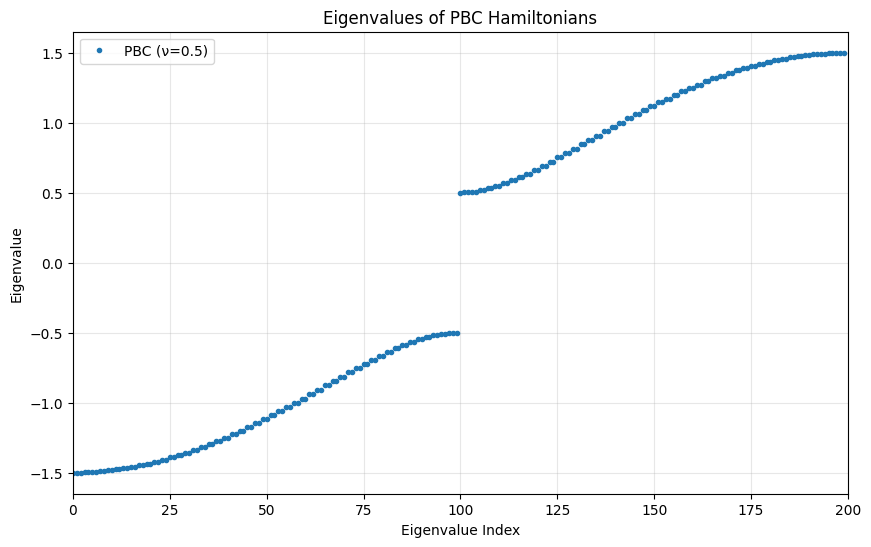
\includegraphics[width=\textwidth]{fig/Question 2/PBC_E_1.png}
        \caption{SSH PBC energy spectrum for $\nu/\omega = 0.5$}
    \end{minipage}
    \hfill
    \begin{minipage}{0.32\textwidth}
        \centering
        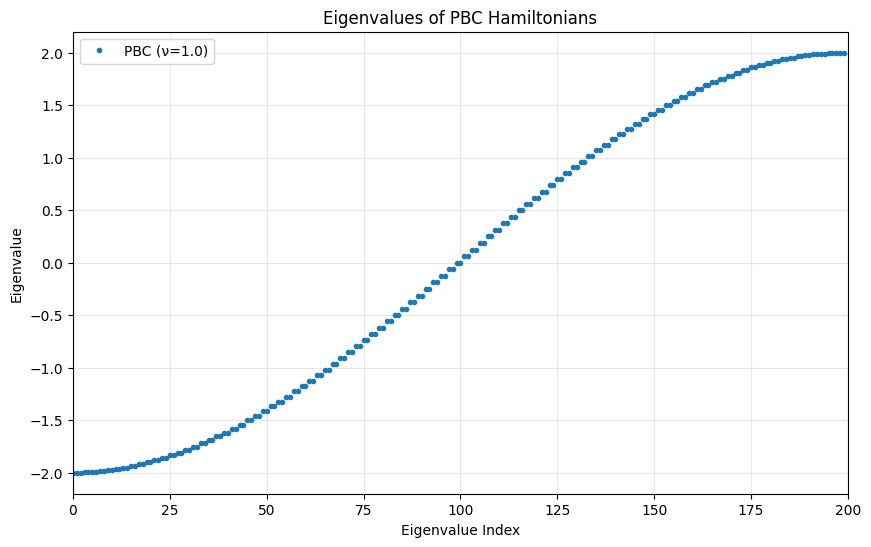
\includegraphics[width=\textwidth]{fig/Question 2/PBC_E_2.png}
        \caption{SSH PBC energy spectrum for $\nu/\omega = 1.0$}
    \end{minipage}
    \hfill
    \begin{minipage}{0.32\textwidth}
        \centering
        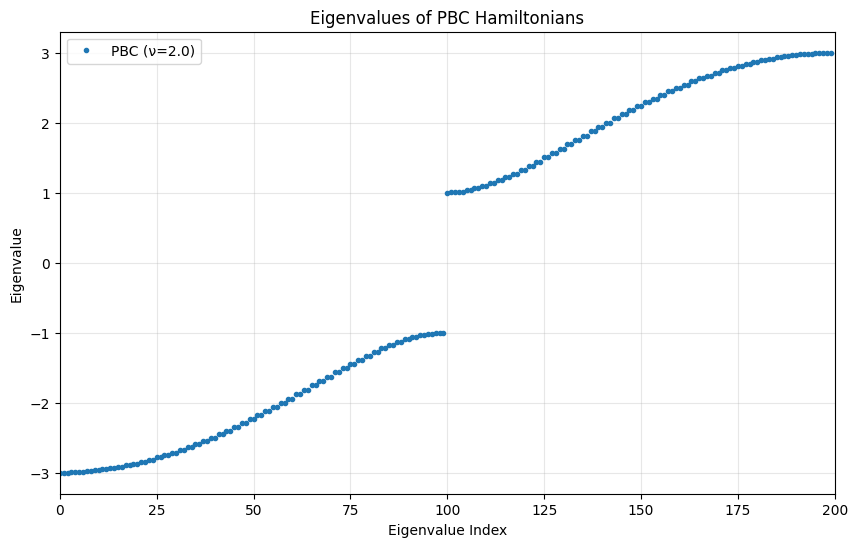
\includegraphics[width=\textwidth]{fig/Question 2/PBC_E_3.png}
        \caption{SSH PBC energy spectrum for $\nu/\omega = 2.0$}
    \end{minipage}

\end{figure}

\nt{$\nu = 1$ corresponds to a metal while $\nu = 0.5$ and $\nu = 2.0$ correspond to insulators. Because the energy bands are gapless for $\nu = 1$ and gapped for $\nu = 0.5$ and $\nu = 2.0$.}

\section{Task 3:  Edge states}
\setcounter{tcb@cnt@question}{0}

\qs{}{Construct the OBC Hamiltonian of the SSH model for $N = 50$ and plot the energy spectrum for different ratios of $\nu/\omega = \{0.5,1,2\}$.}

\sol Calculate the energy spectrum for the open system for $N = 50$ and different values of $\nu/\omega$ and plot the energy spectrum:

\begin{figure}[H]
    \centering

    \begin{minipage}{0.32\textwidth}
        \centering
        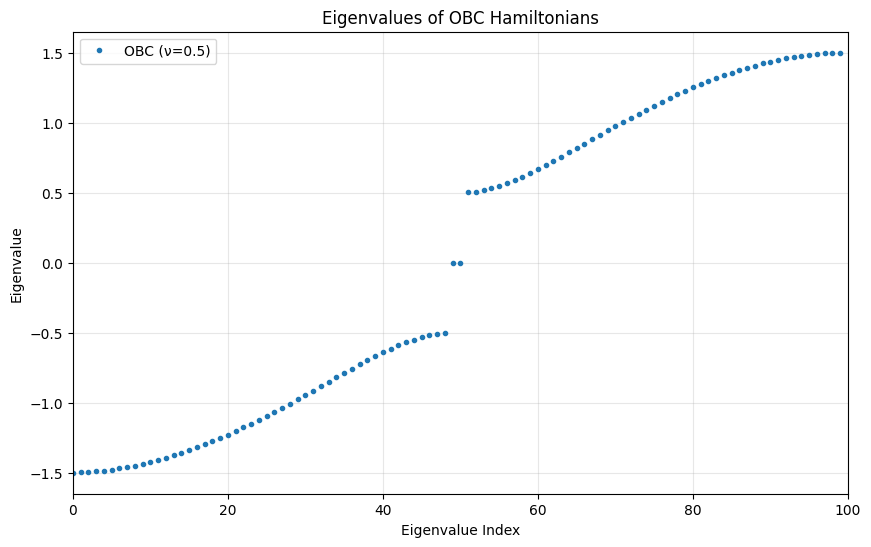
\includegraphics[width=\textwidth]{fig/Question 2/OBC_E_1.png}
        \caption{SSH OBC energy spectrum for $\nu/\omega = 0.5$}
    \end{minipage}
    \hfill
    \begin{minipage}{0.32\textwidth}
        \centering
        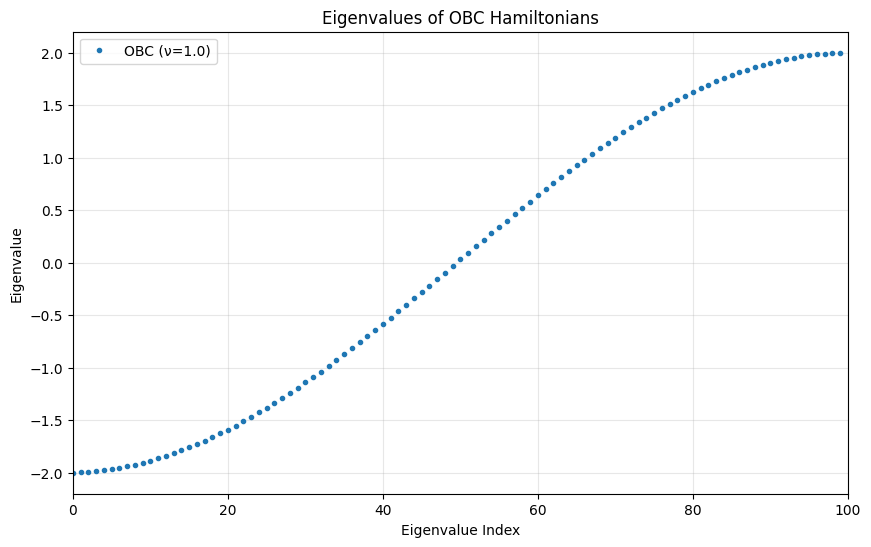
\includegraphics[width=\textwidth]{fig/Question 2/OBC_E_2.png}
        \caption{SSH OBC energy spectrum for $\nu/\omega = 1.0$}
    \end{minipage}
    \hfill
    \begin{minipage}{0.32\textwidth}
        \centering
        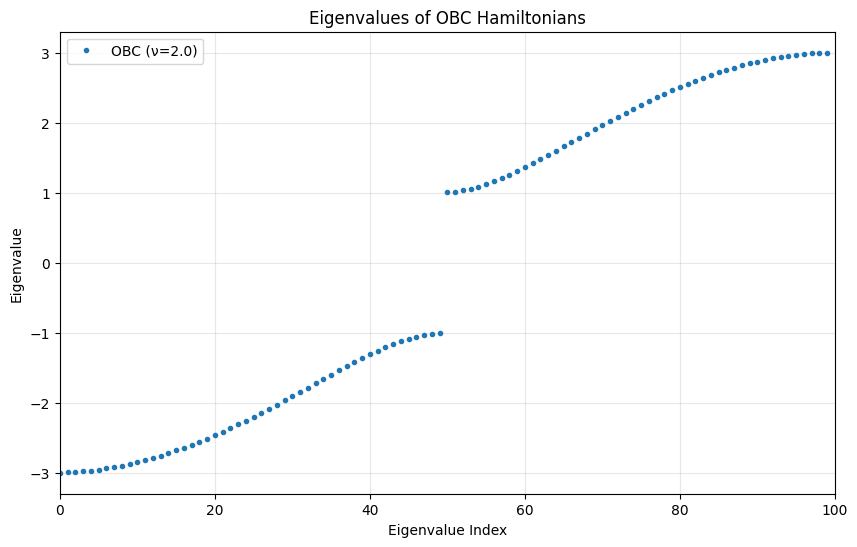
\includegraphics[width=\textwidth]{fig/Question 2/OBC_E_3.png}
        \caption{SSH OBC energy spectrum for $\nu/\omega = 2.0$}
    \end{minipage}
\end{figure}

\begin{question}{}{}
    \begin{itemize}
        \item Identify the zero-energy states for the case when $\nu/\omega = 0.5$. How many are they?
        \item Plot the zero-energy states wavefunctions and verify that they are localized at the boundaries, hence the name ‘edge’ states.
    \end{itemize}
\end{question}

\sol Identify the zero-energy states for the case when $\nu/\omega = 0.5$ using threshold $\epsilon = 1e-10$, and plot the wave functions of the zero-energy states:

\begin{lstlisting}
zero_states = np.where(np.abs(E_OBC_1) < 1e-10)[0]
print("Zero-energy state indices:", zero_states)
print("Number of zero-energy states:", len(zero_states))
print("Energies:", E_OBC_1[zero_states])
\end{lstlisting}

The outputs are as follows:

\begin{lstlisting}
Zero-energy state indices: [49 50]
Number of zero-energy states: 2
Energies: [-9.54080635e-16  3.78186994e-16]
\end{lstlisting}

\nt{The outputs show that there are two zero-energy states for the case when $\nu/\omega = 0.5$.}

Plotting the wave functions of the zero-energy states:

\begin{figure}[H]
    \centering

    \begin{minipage}{0.48\textwidth}
        \centering
        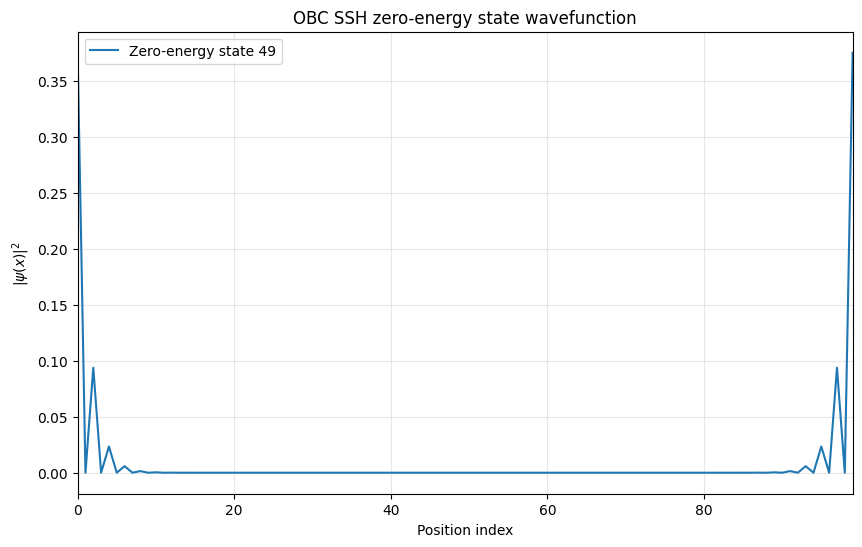
\includegraphics[width=\textwidth]{fig/Question 2/OBC_zero_E_state_1.png}
        \caption{Zero-energy state wavefunction 1}
    \end{minipage}
    \hfill
    \begin{minipage}{0.48\textwidth}
        \centering
        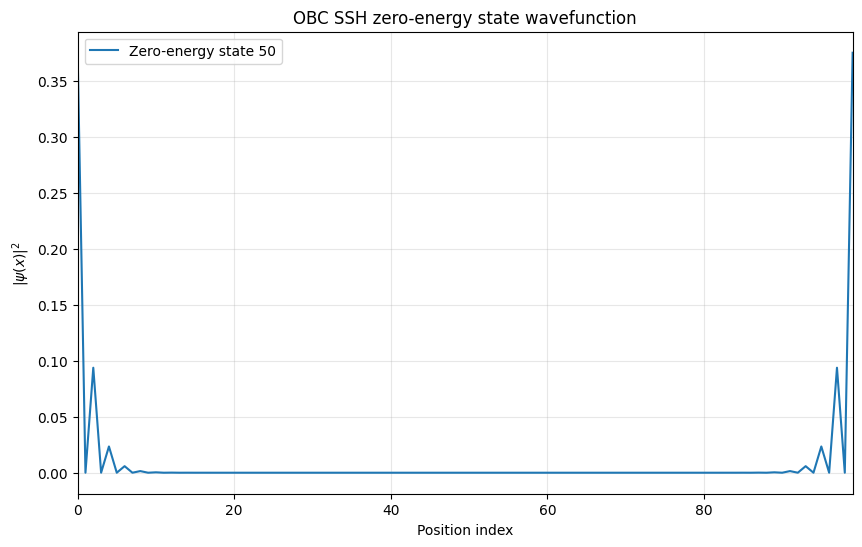
\includegraphics[width=\textwidth]{fig/Question 2/OBC_zero_E_state_2.png}
        \caption{Zero-energy state wavefunction 2}
    \end{minipage}
\end{figure}

\nt{As shown in the plots, the wavefuncitons of zero-energy state are quite localized at the boundaries, which confirms that they are indeed edge states.}

\section{Task 4: Robustness of topological edge states}
\setcounter{tcb@cnt@question}{0}

\begin{question}{}{}
    \begin{itemize}
        \item Add a weak random on-site disorder to your OBC SSH Hamiltonian,

            $$
            H_\text{disorder} = \sum_n \epsilon_{nA} \ket{n; A}\bra{n; A} + \epsilon_{nB} \ket{n; B}\bra{n; B}
            $$

            where $\epsilon_{nA, B}$ are random variables drawn from a uniform distribu1on in the range $[-W,W]$. 

        \item Show that the zero-energy localized states persist for small noise amplitudes $(W < |\omega - \nu|)$ by plotting the spectrum and their wave function probability distribu1ons. For concreteness, use $\nu = 0.5$ and $W = \{0.2,0.4\}$.
    \end{itemize}
\end{question}

\sol Construct the disordered Hamiltonian by adding random on-site disorder to the OBC SSH Hamiltonian:

\begin{lstlisting}
# OBC Hamiltonian for SSH model with disorder
def obc_Hamiltonian_disordered(n, W, nu, omega=1, seed=None):
    H = np.zeros((2 * n, 2 * n))
    rng = np.random.default_rng(seed)
    # SSH Hamiltonian
    for i in range(n):
        H[2 * i + 1, 2 * i] = -nu
        H[2 * i, 2 * i + 1] = -nu
    for i in range(n - 1):
        H[2 * (i + 1), 2 * i + 1] = -omega
        H[2 * i + 1, 2 * (i + 1)] = -omega
    # Disorder term
    for i in range(n):
        H[2 * i, 2 * i] = rng.uniform(-W, W)
        H[2 * i + 1, 2 * i + 1] = rng.uniform(-W, W)

    return H
\end{lstlisting}

Calculate the energy spectrum and wave function probability distributions for the disordered system using the random seed of $67$ for reproducibility:

\begin{lstlisting}
W1 = 0.2
W2 = 0.4
nu = 0.5
N = 100

E1, psi1 = np.linalg.eigh(obc_Hamiltonian_disordered(N, W1, nu, seed=67))
E2, psi2 = np.linalg.eigh(obc_Hamiltonian_disordered(N, W2, nu, seed=67))
\end{lstlisting}

Then we can find the edge states by identifying the eigenvalues that are closest to zero:

\begin{lstlisting}
edge_states_1 = np.argsort(np.abs(E1))[:2]
edge_states_2 = np.argsort(np.abs(E2))[:2]

print("W = 0.2 edge state energies:", E1[edge_states_1])
print("W = 0.4 edge state energies:", E2[edge_states_2])
\end{lstlisting}

The outputs are as follows:

\begin{lstlisting}
W = 0.2 edge state energies: [-0.02428976  0.02461507]
W = 0.4 edge state energies: [-0.04884587  0.05275579]
\end{lstlisting}

\nt{The outputs show that the same edge states in the clean system persist in the presence of disorder, albeit with slightly shifted energies.}

Plotting the energy spectrum and wave function probability distributions for the disordered system:

\begin{figure}[H]
    \centering

    \begin{minipage}{0.48\textwidth}
        \centering
        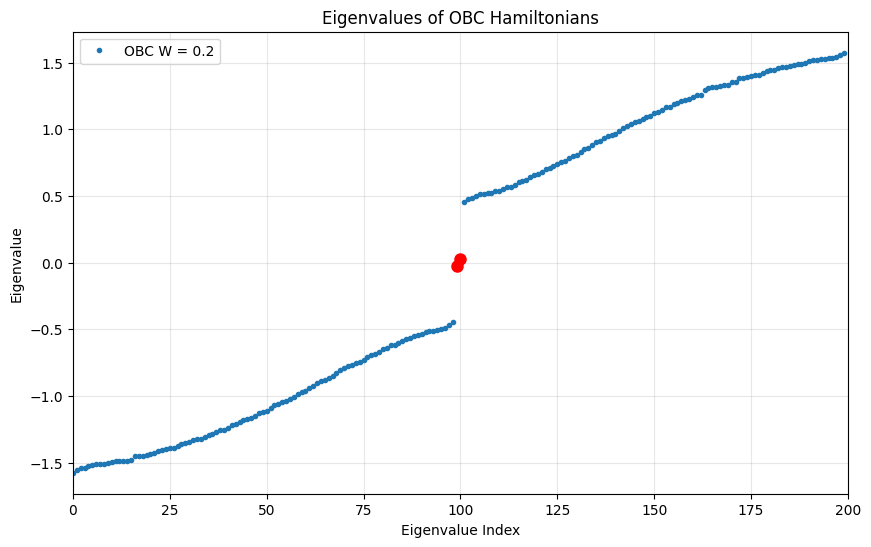
\includegraphics[width=\textwidth]{fig/Question 2/OBC_disordered_zero_E_state_1.png}
        \caption{Energy spectrum for OBC with disorder $W = 0.2$}
    \end{minipage}
    \hfill
    \begin{minipage}{0.48\textwidth}
        \centering
        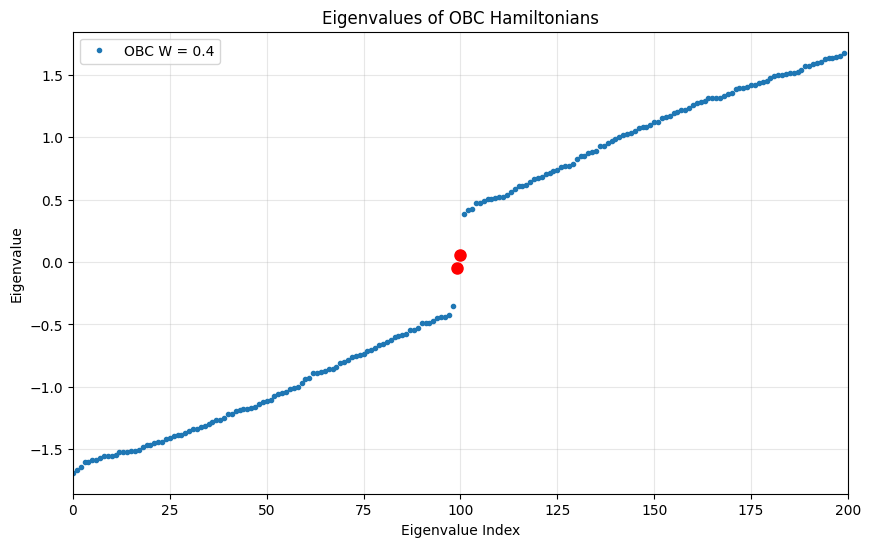
\includegraphics[width=\textwidth]{fig/Question 2/OBC_disordered_zero_E_state_2.png}
        \caption{Energy spectrum for OBC with disorder $W = 0.4$}
    \end{minipage}
\end{figure}

\nt{These plots shows that bigger disorder strength leads to larger energy shifts for the edge states, but they still persist as long as the disorder strength is smaller than the bulk gap.}

Plotting the wave function probability distributions for the edge states in the disordered system:

\begin{figure}[H]
    \centering

    \begin{minipage}{0.48\textwidth}
        \centering
        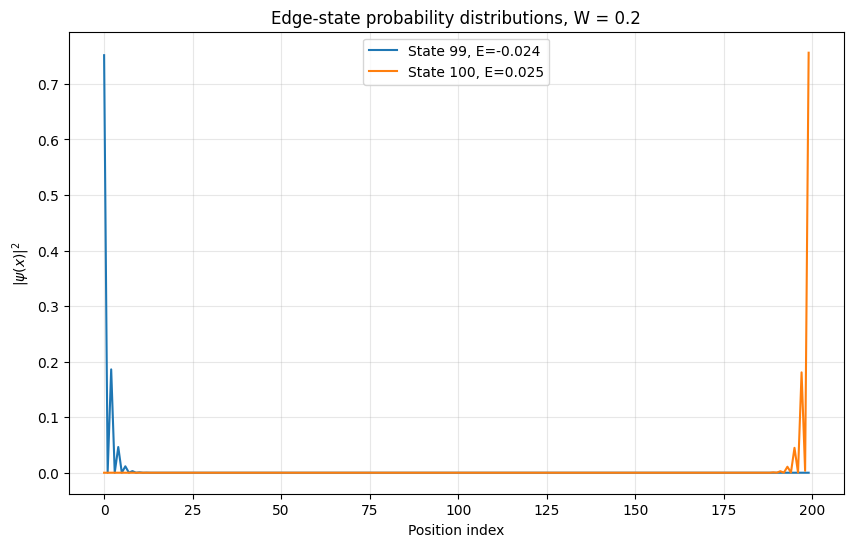
\includegraphics[width=\textwidth]{fig/Question 2/OBC_disordered_zero_E_state_wavefunction_1.png}
        \caption{Edge state probability distribution for $W = 0.2$}
    \end{minipage}
    \hfill
    \begin{minipage}{0.48\textwidth}
        \centering
        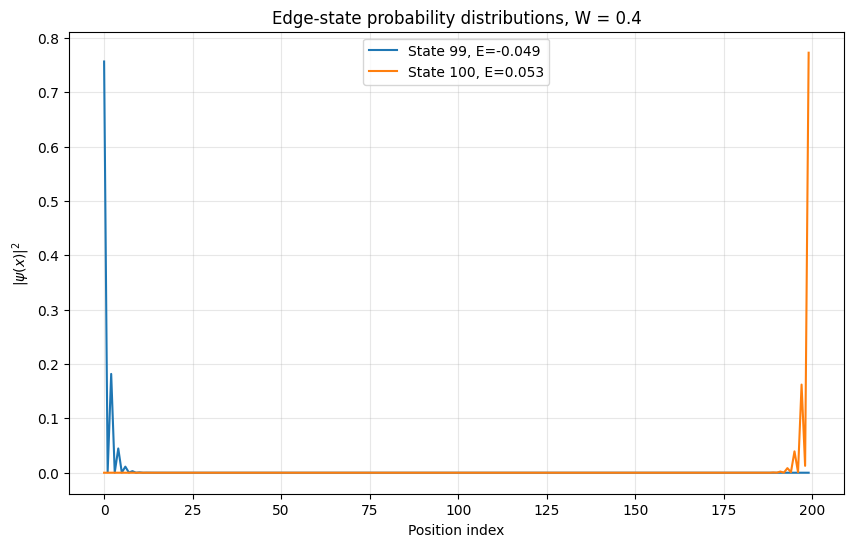
\includegraphics[width=\textwidth]{fig/Question 2/OBC_disordered_zero_E_state_wavefunction_2.png}
        \caption{Edge state probability distribution for $W = 0.4$}
    \end{minipage}
\end{figure}

\appendix
\chapter*{Appendix}
\addcontentsline{toc}{chapter}{Appendix}

I used Jupyter Notebook to finish the coding of this project and have uploaded the notebook to GitHub. You can find it at the following link \url{https://github.com/zengxuanliu2005/Solid_State_Physics_Project}. Also my git commit history is available at the same repository.

Complete code for this project will be provided as follows for reference. Since I use Jupyter Notebook to finish the coding of this project, all codes will be presented here in the form of cells.

\section*{Importing necessary libraries}

\begin{lstlisting}
import numpy as np
import matplotlib.pyplot as plt
import scipy
\end{lstlisting}

\section*{Simple tight-binding model code}
\subsection*{Task 1: Hamiltonian construction}

\begin{lstlisting}
# PBC 
def pbc_Hamiltonian(n, t = 1):
    H = np.zeros((n, n))
    for i in range(n):
        H[i, (i + 1) % n] = -t
        H[(i + 1) % n, i] = -t
    return H

# OBC
def obc_Hamiltonian(n, t = 1):
    H = np.zeros((n, n))
    for i in range(n - 1):
        H[i, i + 1] = -t
        H[i + 1, i] = -t
    return H
\end{lstlisting}

\begin{lstlisting}
# Example
N = 5
H_PBC = pbc_Hamiltonian(N)
H_OBC = obc_Hamiltonian(N)

print("Hamiltonian in PBC:")
print(H_PBC)
print(scipy.linalg.ishermitian(H_PBC))
print("Hamiltonian in OBC:")
print(H_OBC)
print(scipy.linalg.ishermitian(H_OBC))
\end{lstlisting}

\subsection*{Task 2: Eigenvalue problem}

\begin{lstlisting}
# Diagonalize
N = 100
E_PBC, psi_PBC = np.linalg.eigh(pbc_Hamiltonian(N))
E_OBC, psi_OBC = np.linalg.eigh(obc_Hamiltonian(N))
\end{lstlisting}

\begin{lstlisting}
plt.figure(figsize=(10, 6))
N = 100

plt.plot(E_PBC, 'o', label='PBC', markersize=3, color='blue')
plt.plot(E_OBC, 's', label='OBC', markersize=3, color='red')
plt.xlabel('Eigenvalue Index')
plt.ylabel('Eigenvalue')
plt.title('Eigenvalues of PBC and OBC Hamiltonians')
plt.legend(loc='upper left')
plt.grid(True, alpha = 0.3)
plt.xlim(0, N)
plt.show()
\end{lstlisting}

\begin{lstlisting}
# Ground state and first two excited state probability plots
def plot_ground_and_excited_states(N, E, psi, title):
    x = np.arange(N)

    psi_gs = psi[:, 0]   # ground state
    psi_e1 = psi[:, 1]   # first excited state
    psi_e2 = psi[:, 2]   # second excited state

    plt.figure(figsize=(10, 6))
    plt.plot(x, np.abs(psi_gs)**2, label=f"{'Ground state':} E = {E[0]:.3f}", color="blue")
    plt.plot(x, np.abs(psi_e1)**2, label=f"{'1st excited state':} E = {E[1]:.3f}", color="orange")
    plt.plot(x, np.abs(psi_e2)**2, label=f"{'2nd excited state':} E = {E[2]:.3f}", color="red")

    plt.xlabel("Position index")
    plt.ylabel(r"$|\psi(x)|^2$")
    plt.xlim(0, N-1)
    plt.title(title)
    plt.legend(loc="upper right")
    plt.grid(True, alpha=0.3)
    plt.show()

plot_ground_and_excited_states(N, E_PBC, psi_PBC, "PBC probability distributions")
plot_ground_and_excited_states(N, E_OBC, psi_OBC, "OBC probability distributions")
\end{lstlisting}

\section*{SSH model code}
\subsection*{Task 1: Hamiltonian construction}

\begin{lstlisting}
# PBC 
def pbc_Hamiltonian(n, nu, omega = 1):
    H = np.zeros((2 * n, 2 * n))
    for i in range(n):
        H[2 * i + 1, 2 * i] = -nu
        H[2 * i, 2 * i + 1] = -nu
        H[2 * (i + 1) % (2 * n), 2 * i + 1] = -omega
        H[2 * i + 1, 2 * (i + 1) % (2 * n)] = -omega
    return H

# OBC
def obc_Hamiltonian(n, nu, omega=1):
    H = np.zeros((2 * n, 2 * n))
    for i in range(n):
        H[2 * i + 1, 2 * i] = -nu
        H[2 * i, 2 * i + 1] = -nu
    for i in range(n - 1):
        H[2 * (i + 1), 2 * i + 1] = -omega
        H[2 * i + 1, 2 * (i + 1)] = -omega
    return H
\end{lstlisting}

\subsection*{Task 2: Bulk band structure}

\begin{lstlisting}
# Diagonalize
N = 100
nu_1 = 0.5
nu_2 = 1
nu_3 = 2
omega = 1
E_PBC_1, psi_PBC_1 = np.linalg.eigh(pbc_Hamiltonian(N, nu_1, omega))
E_PBC_2, psi_PBC_2 = np.linalg.eigh(pbc_Hamiltonian(N, nu_2, omega))
E_PBC_3, psi_PBC_3 = np.linalg.eigh(pbc_Hamiltonian(N, nu_3, omega))
\end{lstlisting}

\begin{lstlisting}
N = 100
plt.figure(figsize=(10, 6))

plt.plot(E_PBC_1, 'o', markersize=3, label='PBC (ν=0.5)')
plt.xlabel('Eigenvalue Index')
plt.ylabel('Eigenvalue')
plt.title('Eigenvalues of PBC Hamiltonians')
plt.legend(loc='upper left')
plt.grid(True, alpha = 0.3)
plt.xlim(0, 2 * N)
plt.show()

plt.figure(figsize=(10, 6))

plt.plot(E_PBC_2, 'o', markersize=3, label='PBC (ν=1.0)')
plt.xlabel('Eigenvalue Index')
plt.ylabel('Eigenvalue')
plt.title('Eigenvalues of PBC Hamiltonians')
plt.legend(loc='upper left')
plt.grid(True, alpha = 0.3)
plt.xlim(0, 2 * N)
plt.show()

plt.figure(figsize=(10, 6))

plt.plot(E_PBC_3, 'o', markersize=3, label='PBC (ν=2.0)')
plt.xlabel('Eigenvalue Index')
plt.ylabel('Eigenvalue')
plt.title('Eigenvalues of PBC Hamiltonians')
plt.legend(loc='upper left')
plt.grid(True, alpha = 0.3)
plt.xlim(0, 2 * N)
plt.show()
\end{lstlisting}

\subsection*{Task 3: Edge states}

\begin{lstlisting}
# Diagonalize
N = 50
nu1 = 0.5
nu2 = 1
nu3 = 2
omega = 1
E_OBC_1, psi_OBC_1 = np.linalg.eigh(obc_Hamiltonian(N, nu1, omega))
E_OBC_2, psi_OBC_2 = np.linalg.eigh(obc_Hamiltonian(N, nu2, omega))
E_OBC_3, psi_OBC_3 = np.linalg.eigh(obc_Hamiltonian(N, nu3, omega))
\end{lstlisting}

\begin{lstlisting}
plt.figure(figsize=(10, 6))
N = 50

plt.plot(E_OBC_1, 'o', markersize=3, label='OBC (ν=0.5)')
plt.xlabel('Eigenvalue Index')
plt.ylabel('Eigenvalue')
plt.title('Eigenvalues of OBC Hamiltonians')
plt.legend(loc='upper left')
plt.grid(True, alpha = 0.3)
plt.xlim(0, 2 * N)
plt.show()

plt.figure(figsize=(10, 6))

plt.plot(E_OBC_2, 'o', markersize=3, label='OBC (ν=1.0)')
plt.xlabel('Eigenvalue Index')
plt.ylabel('Eigenvalue')
plt.title('Eigenvalues of OBC Hamiltonians')
plt.legend(loc='upper left')
plt.grid(True, alpha = 0.3)
plt.xlim(0, 2 * N)
plt.show()

plt.figure(figsize=(10, 6))

plt.plot(E_OBC_3, 'o', markersize=3, label='OBC (ν=2.0)')
plt.xlabel('Eigenvalue Index')
plt.ylabel('Eigenvalue')
plt.title('Eigenvalues of OBC Hamiltonians')
plt.legend(loc='upper left')
plt.grid(True, alpha = 0.3)
plt.xlim(0, 2 * N)
plt.show()
\end{lstlisting}

\begin{lstlisting}
zero_states = np.where(np.abs(E_OBC_1) < 1e-10)[0]
print("Zero-energy state indices:", zero_states)
print("Number of zero-energy states:", len(zero_states))
print("Energies:", E_OBC_1[zero_states])
\end{lstlisting}

\begin{lstlisting}
x = np.arange(2 * N)
for i in zero_states:
    prob = np.abs(psi_OBC_1[:, i])**2
    plt.figure(figsize=(10, 6))
    plt.plot(x, prob, label=f"Zero-energy state {i}")

    plt.xlabel("Position index")
    plt.ylabel(r"$|\psi(x)|^2$")
    plt.title("OBC SSH zero-energy state wavefunction")
    plt.legend(loc="upper left")
    plt.grid(True, alpha=0.3)
    plt.xlim(0, 2 * N - 1)
    plt.show()
\end{lstlisting}

\subsection*{Task 4: Robustness of topological edge states}

\begin{lstlisting}
# OBC Hamiltonian for SSH model with disorder
def obc_Hamiltonian_disordered(n, W, nu, omega=1, seed=None):
    H = np.zeros((2 * n, 2 * n))
    rng = np.random.default_rng(seed)
    # SSH Hamiltonian
    for i in range(n):
        H[2 * i + 1, 2 * i] = -nu
        H[2 * i, 2 * i + 1] = -nu
    for i in range(n - 1):
        H[2 * (i + 1), 2 * i + 1] = -omega
        H[2 * i + 1, 2 * (i + 1)] = -omega
    # Disorder term
    for i in range(n):
        H[2 * i, 2 * i] = rng.uniform(-W, W)
        H[2 * i + 1, 2 * i + 1] = rng.uniform(-W, W)

    return H
\end{lstlisting}

\begin{lstlisting}
W1 = 0.2
W2 = 0.4
nu = 0.5
N = 100

E1, psi1 = np.linalg.eigh(obc_Hamiltonian_disordered(N, W1, nu, seed=67))
E2, psi2 = np.linalg.eigh(obc_Hamiltonian_disordered(N, W2, nu, seed=67))
\end{lstlisting}

\begin{lstlisting}
edge_states_1 = np.argsort(np.abs(E1))[:2]
edge_states_2 = np.argsort(np.abs(E2))[:2]

print("W = 0.2 edge state energies:", E1[edge_states_1])
print("W = 0.4 edge state energies:", E2[edge_states_2])
\end{lstlisting}

\begin{lstlisting}
plt.figure(figsize=(10, 6))
N = 100

plt.plot(E1, 'o', markersize=3, label="OBC W = 0.2")
plt.plot(edge_states_1, E1[edge_states_1], "ro", markersize=8)
plt.xlabel('Eigenvalue Index')
plt.ylabel('Eigenvalue')
plt.title('Eigenvalues of OBC Hamiltonians')
plt.legend(loc='upper left')
plt.grid(True, alpha = 0.3)
plt.xlim(0, 2 * N)
plt.show()

plt.figure(figsize=(10, 6))

plt.plot(E2, 'o', markersize=3, label="OBC W = 0.4")
plt.plot(edge_states_2, E2[edge_states_2], "ro", markersize=8)
plt.xlabel('Eigenvalue Index')
plt.ylabel('Eigenvalue')
plt.title('Eigenvalues of OBC Hamiltonians')
plt.legend(loc='upper left')
plt.grid(True, alpha = 0.3)
plt.xlim(0, 2 * N)
plt.show()
\end{lstlisting}

\begin{lstlisting}
x = np.arange(2 * N)

for W, E, psi, edge_states in [
    (0.2, E1, psi1, edge_states_1),
    (0.4, E2, psi2, edge_states_2),
]:
    plt.figure(figsize=(10, 6))

    for idx in edge_states:
        plt.plot(x, np.abs(psi[:, idx])**2, label=f"State {idx}, E={E[idx]:.3f}")

    plt.xlabel("Position index")
    plt.ylabel(r"$|\psi(x)|^2$")
    plt.title(f"Edge-state probability distributions, W = {W}")
    plt.legend()
    plt.grid(True, alpha=0.3)
    plt.show()
\end{lstlisting}

\end{document}
